% !TeX root = ../quantum.tex
\chapter{امنیت لایه فیزیکی}
\label{chap:4}

\section*{چکیده}
این فصل به امنیت لایه فیزیکی (\lr{PLS}) اختصاص یافته است. فصل با بحثی درباره مسائل امنیتی آغاز شده و با مقدمه‌ای بر امنیت نظریه-اطلاعاتی\LTRfootnote{Information-theoretic security} و مقایسه آن با امنیت محاسباتی\LTRfootnote{Computational security} ادامه می‌یابد. در همان بخش، معیارهای مختلف امنیت نظریه-اطلاعاتی، از جمله شرایط محرمانگی قوی\LTRfootnote{Strong secrecy} و ضعیف\LTRfootnote{Weak secrecy} معرفی می‌شوند. سپس، مدل کانال شنود\LTRfootnote{Wiretap channel} واینر\LTRfootnote{Wyner} که با نام مدل کانال شنود تخریب‌شده\LTRfootnote{Degraded wiretap channel} نیز شناخته می‌شود، معرفی می‌گردد. در همان بخش، مفهوم ظرفیت محرمانگی\LTRfootnote{Secrecy capacity} و همچنین کدگذاری شنود آشیانه‌ای\LTRfootnote{Nested wiretap coding} بررسی می‌شود. علاوه بر این، کانال پخش با پیام‌های محرمانه\LTRfootnote{Broadcast channel with confidential messages} معرفی شده و تعریف ظرفیت محرمانگی تعمیم می‌یابد. سپس تمرکز به سمت تولید (توافق) کلید مخفی\LTRfootnote{Secret-key generation (agreement)} معطوف شده، مدل‌های نوع منبع و نوع کانال معرفی می‌شوند و پروتکل‌های تولید کلید مخفی متناظر تشریح می‌گردند. بخش بعدی به کدگذاری برای سیستم‌های امنیت لایه فیزیکی، شامل کدگذاری برای هر دو سیستم محرمانگی ضعیف و قوی اختصاص دارد. در رابطه با کدگذاری برای سیستم‌های محرمانگی ضعیف، توجه ویژه‌ای به کدگذاری \lr{LDPC} نوع دو-لبه\LTRfootnote{Two-edge-type LDPC coding}، کدگذاری \lr{LDPC} پنچرشده\LTRfootnote{Punctured LDPC coding} و کدهای قطبی\LTRfootnote{Polar codes} معطوف شده است. در مورد کدگذاری برای سیستم‌های محرمانگی قوی، تمرکز بر کدگذاری هم‌مجموعه‌ای\LTRfootnote{Coset coding} با کدهای \lr{LDPC} دوگان و کدگذاری مبتنی بر توابع هش/استخراج‌کننده\LTRfootnote{Hash functions/extractor-based coding} است. سپس بحث به سمت مصالحه اطلاعات\LTRfootnote{Information reconciliation} و تقویت حریم خصوصی\LTRfootnote{Privacy amplification} حرکت می‌کند. در بخش امنیت لایه فیزیکی کانال‌های بی‌سیم، موضوعات زیر پوشش داده می‌شوند: مبانی \lr{MIMO}، \lr{PLS} در سیستم‌های \lr{MIMO} بی‌سیم، و تولید کلید مخفی در شبکه‌های بی‌سیم. در بخش \lr{PLS} کانال‌های نوری، هر دو حوزه \lr{PLS} برای سیستم‌های مبتنی بر فیبرهای تسهیم‌سازی تقسیم فضایی\LTRfootnote{Spatial division multiplexing (SDM)} و سیستم‌های نوری فضای آزاد (\lr{FSO}) مورد بحث قرار می‌گیرند.







\section{مسائل امنیتی}
\label{sec:4-1}
رمزنگاری کلید عمومی\LTRfootnote{Public key cryptography} دارای چندین نقص جدی است؛ از جمله اینکه پیاده‌سازی آن در دستگاه‌هایی با حافظه کم و محدودیت‌های پردازشی پایین دشوار است، اینترنت به‌طور فزاینده‌ای در حال متحرک شدن است، طرح‌های امنیتی بر پایه فرضیات اثبات‌نشده‌ای از دشواری\LTRfootnote{Intractability} توابع خاص بنا شده‌اند، و فرضِ محدود بودن منابع محاسباتی ایو\LTRfootnote{Eve} همیشه صادق نیست. مدل مرجع اتصال متقابل سیستم‌های باز\LTRfootnote{Open-system interconnection (OSI)} (\lr{OSI}) هفت لایه را تعریف می‌کند. با این حال، در شکل \ref{fig:4-1} تنها پنج لایه مرتبط با مسائل امنیتی ارائه شده است. مدل اصلی \lr{OSI} اصلاً مسائل امنیتی را مشخص نمی‌کند. این مسائل در استاندارد \lr{X.800} (معماری امنیتی برای \lr{OSI}) مورد توجه قرار گرفته‌اند \cite{4-1}. اگرچه امنیت لایه فیزیکی\LTRfootnote{Physical-layer security (PLS)} (\lr{PLS}) در این استاندارد مورد بحث قرار نگرفته است، اما همان‌طور که در مراجع \cite{4-2, 4-3, 4-4} بحث شده، سرویس‌های مشخص‌شده در این پنج لایه را می‌توان با به‌کارگیری \lr{PLS} بهبود بخشید. طرح \lr{PLS} می‌تواند به‌صورت مستقل نیز عمل کند. از اعوجاج‌ها و اثرات نویزی وارد شده توسط کانال می‌توان برای کاهش تعداد بیت‌های استخراج شده توسط ایو بهره‌برداری کرد. در مقایسه با رویکردهای رمزنگاری متداول که در آن‌ها از طرح‌های کدگذاری کنترل خطا\LTRfootnote{Error control coding (ECC)} (\lr{ECC}) قوی برای فراهم‌سازی ارتباطات قابل‌اطمینان استفاده می‌شود، ارسال در سناریوی \lr{PLS} باید به‌طور هم‌زمان قابل‌اطمینان و امن باشد. این امر نشان می‌دهد که باید کلاس‌های متفاوتی از \lr{ECC} توسعه یابند؛ این کدها در ادامه این فصل مورد بحث قرار خواهند گرفت. متناوباً، مشابه با توزیع کلید کوانتومی\LTRfootnote{Quantum key distribution (QKD)} (\lr{QKD})، می‌توان از تصادفی بودن کانال برای تولید کلید بهره‌برداری کرد؛ این رویکرد معمولاً با عنوان توافق کلید مخفی\LTRfootnote{Secret-key agreement} شناخته می‌شود و این مفهوم در شکل \ref{fig:4-2} با الهام از مراجع \cite{4-2, 4-3, 4-6} توصیف شده است.

\begin{figure}[ht]
	\centering
	 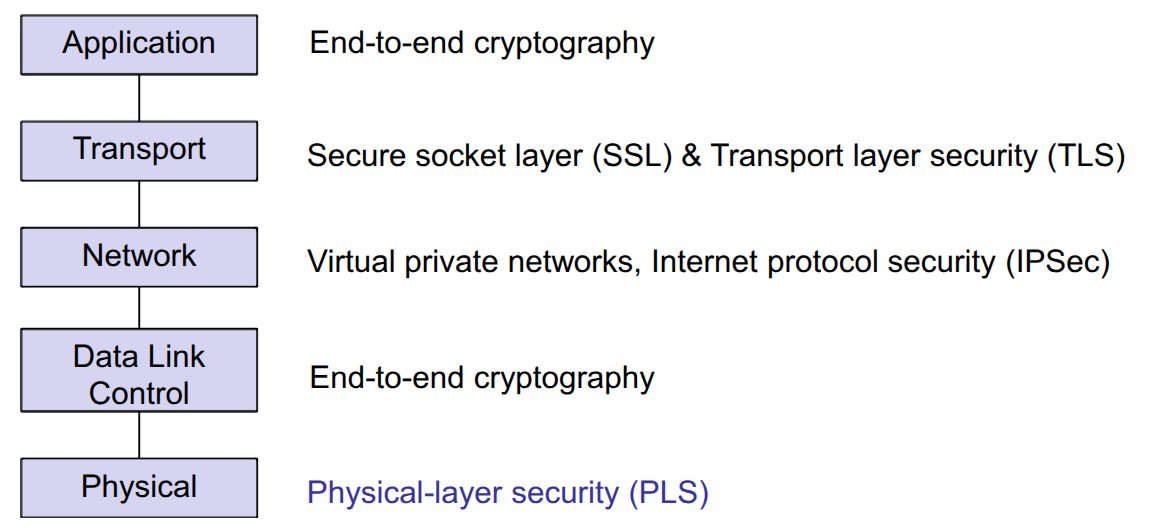
\includegraphics[width=0.8\textwidth]{chapters/figs/fig-4-1}
	\caption{مکانیزم‌های امنیتی در لایه‌های مختلف مدل \lr{OSI}. (تنها لایه‌های مرتبط با امنیت نشان داده شده‌اند)}
	\label{fig:4-1}
\end{figure}

آلیس و باب ظرفیت کانال آلیس-باب (که با نام ظرفیت کانال اصلی\LTRfootnote{Capacity of the main channel} نیز شناخته می‌شود) $C_M$ و ظرفیت محرمانگی\LTRfootnote{Secrecy capacity} $C_S$ را، که به‌صورت تفاضل بین ظرفیت کانال اصلی و ظرفیت کانال شنود\LTRfootnote{Eavesdropping channel capacity} $C_E$ تعریف می‌شود، پایش می‌کنند. زمانی که ظرفیت محرمانگی به‌میزان کافی بالاتر از مقدار آستانه $C_{S,tsh}$ و ظرفیت کانال اصلی به‌خوبی بالاتر از مقدار آستانه $C_{M,tsh}$ باشد، آلیس نمادهای با شکل گاوسی\LTRfootnote{Gaussian-shaped symbols} $X$ را برای باب ارسال می‌کند. هنگامی که هر دو ظرفیت محرمانگی و ظرفیت کانال اصلی به دلیل محوشدگی عمیق\LTRfootnote{Deep fading} پایین‌تر از آستانه‌های مربوطه قرار گیرند، آلیس و باب مصالحه اطلاعات\LTRfootnote{Information reconciliation} نمادهای ارسال‌شده قبلی را انجام می‌دهند که بر پایه طرح \lr{ECC} قوی است تا اطمینان حاصل شود که خطاهای وارد شده توسط کانال یا ایو قابل اصلاح هستند. مشابه با طرح‌های \lr{QKD} \cite{4-7, 4-8, 4-9, 4-10, 4-11, 4-12, 4-13, 4-14}، می‌توان از یک کد بررسی توازن کم‌چگال (\lr{LDPC})\LTRfootnote{Low-density parity-check (LDPC)} سیستماتیک استفاده کرد (که بر بیت‌های اطلاعات تأثیری نمی‌گذارد اما بیت‌های بررسی توازن را که به‌صورت جبری با بیت‌های اطلاعات مرتبط هستند تولید می‌کند) تا بیت‌های توازن را تولید کرده و آن‌ها را از طریق یک کانال عمومی احرازهویت‌شده ارسال نماید. طرح‌های مصالحه اطلاعات مستقیم و معکوس وجود دارند. در مصالحه مستقیم، که در شکل \ref{fig:4-2} نشان داده شده است، آلیس رمزگذاری \lr{LDPC} را انجام داده و بیت‌های توازن را برای باب ارسال می‌کند. باب رمزگشایی \lr{LDPC} را برای به‌دست آوردن کلید صحیح $X$ انجام می‌دهد. در مصالحه معکوس، باب به جای آلیس رمزگذاری \lr{LDPC} را انجام می‌دهد. سپس تقویت حریم خصوصی\LTRfootnote{Privacy amplification} بین آلیس و باب انجام می‌شود تا از $X$ مجموعه کوچک‌تری از بیت‌های $K$ (کلید امن\LTRfootnote{Secure key}) استخراج گردد که همبستگی آن با رشته ایو پایین‌تر از یک آستانه مطلوب باشد. یکی از راه‌های انجام تقویت حریم خصوصی، استفاده از توابع هش سراسری\LTRfootnote{Universal hash functions} $G$ \cite{4-9, 4-12, 4-14, 4-15} است، که مجموعه رشته‌های $n$-بیتی $X$ را به مجموعه رشته‌های $m$-بیتی $K$ نگاشت می‌کنند، به‌طوری که برای هر دو رشته متمایز $X_1$ و $X_2$ از مجموعه کلیدهای اصلاح‌شده، زمانی که نگاشت $g$ به‌صورت یکنواخت و تصادفی از $G$ انتخاب شود، احتمال برقراری $g(X_1) = g(X_2)$ بسیار پایین باشد.




\begin{figure}[ht]
	\centering
	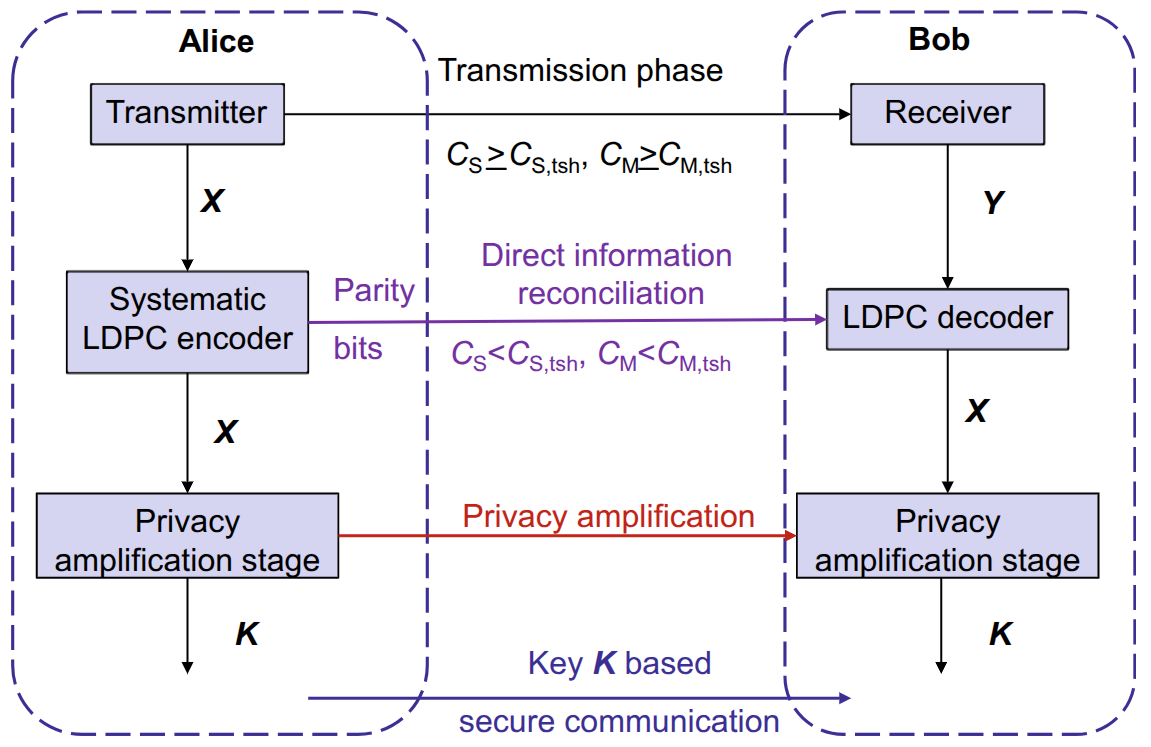
\includegraphics[width=0.8\textwidth]{chapters/figs/fig-4-2}
	\caption{پروتکل تولید (توافق) کلید مخفی مناسب برای مخابرات بی‌سیم.}
	\label{fig:4-2}
\end{figure}

\begin{figure}[ht]
	\centering
	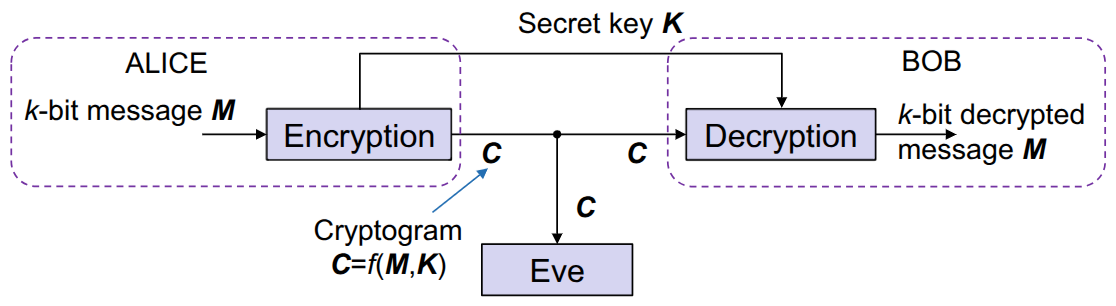
\includegraphics[width=0.8\textwidth]{chapters/figs/fig-4-3}
	\caption{مدل شانون برای سیستم محرمانگی.}
	\label{fig:4-3}
\end{figure}

\section{امنیت نظریه-اطلاعاتی در مقابل امنیت محاسباتی}
\label{sec:4-2}
مدل شانون برای سیستم محرمانگی \cite{4-16} در شکل \ref{fig:4-3} به تصویر کشیده شده است. هدف از این سیستم، ارسال قابل‌اطمینان پیام $M$ است که به‌طور هم‌زمان از دیدگاه ایو محرمانه باشد. برای انجام این کار، آلیس و باب به کلید تصادفی $K$ دسترسی دارند که برای ایو ناشناخته است و توسط آلیس برای رمزگذاری پیام به رمزنگاشت $C$ استفاده می‌شود. در سمت گیرنده، باب رمزنگاشت $C$ را با کمک کلید $K$ رمزگشایی کرده و پیام ارسالی $M$ را تعیین می‌کند.

\subsection{امنیت نظریه-اطلاعاتی (کامل)}
\label{subsec:4-2-1}
ما می‌گوییم پیام با امنیت کامل\LTRfootnote{Perfect security} ارسال شده است اگر دانش ایو درباره رمزنگاشت به او در رمزگشایی پیام کمکی نکند. به عبارت دیگر، $Pr(M | \text{Eve's knowledge}) = Pr(M)$. به‌وضوح، در مفهوم امنیت کامل، کلمه کد $C$ از نظر آماری مستقل از پیام $M$ است و می‌توانیم بنویسیم $H(M|C) = H(M)$. به‌طور معادل، اطلاعات متقابل بین کلمه کد $C$ و پیام $M$ صفر است، یعنی $I(M;C) = H(M|C) - H(M) = 0$. در این سناریو، بهترین استراتژی برای ایو حدس زدن پیام است که احتمال موفقیت آن $2^{-k}$ بوده و با افزایش طول کلید $k$ به‌صورت نمایی کاهش می‌یابد. با به‌کارگیری قاعده زنجیره‌ای\LTRfootnote{Chain rule} از فصل \ref{chap:2}، می‌توانیم بنویسیم:
\begin{equation}
	H(M) = H(M|C) \leq H(M, K|C) = H(K|C) + \underbrace{H(M|C, K)}_{0} = H(K|C) \leq H(K),
	\label{eq:4-1}
\end{equation}
که در آن از این واقعیت استفاده کردیم که وقتی هم رمزنگاشت و هم کلید معلوم باشند، پیام کاملاً مشخص می‌شود، یعنی $H(M|K, C) = 0$. بنابراین، شرط محرمانگی کامل به‌صورت زیر داده می‌شود:
\begin{equation}
	H(M) \leq H(K).
	\label{eq:4-2}
\end{equation}
در نتیجه، برای اینکه یک طرح رمزگذاری دارای امنیت کامل باشد، آنتروپی (عدم قطعیت) کلید نمی‌تواند کمتر از آنتروپی پیام باشد.